%%====================================================================%%
%%                	AGH University of Science and Technology
%%	Faculty of Electrical Engineering, Automatics, IT and Electronics
%%			Department of Computer Science
%%				Master's thesis
%%
%%            Author : Adrian Wolny
%%        Speciality : Distributed systems and computer networks
%%      Register No. : 203789
%% Thesis Supervisor : Prof. dr hab. in�. Robert Schaefer
%%    Date (version) : 01.06.2011 0.1
%%
%%--------------------------------------------------------------------%%

\documentclass[pdflatex,11pt]{aghdpl}
%%\usepackage[polish]{babel}
\usepackage[utf8]{inputenc}
\usepackage{amsthm}
\usepackage{enumerate}
%%\usepackage{minted}
\usepackage{array}

\graphicspath{{./img/}}

\theoremstyle{definition}
%%\newtheorem{przyklad}{Przyk�ad}

%%\newminted{java}{gobble=4, linenos, numbersep=8pt}
%%\newminted{js}{gobble=4, linenos, numbersep=8pt}
%%\newminted{xml}{gobble=4, linenos, numbersep=8pt}
%%\renewcommand{\theFancyVerbLine}{\ttfamily\small\oldstylenums{\arabic{FancyVerbLine}}}

%---------------------------------------------------------------------------

\author{Adrian Wolny}
\shortauthor{A. Wolny}

%%\titlePL{Poprawa algoryt�w populacyjnych w problemach optymalizacji globalnej
%%poprzez deterioracj� funkcji przystosowania}
\titleEN{Improving population-based algorithms used in Global Optimization with
Fitness Deterioration techniques}

%%\thesistypePL{Praca magisterska}
\thesistypeEN{Master of Science Thesis}

%%\supervisorPL{Prof. dr hab. in�. Robert Schaefer}
\supervisorEN{Robert Schaefer, Prof., PhD, DSc}

\date{2011}

%%\departmentPL{Katedra Informatyki}
\departmentEN{Department of Computer Science}

%%\facultyPL{Wydzia� Elektrotechniki, Automatyki, Informatyki i Elektroniki}
\facultyEN{Faculty of Electrical Engineering, Automatics, Computer Science and Electronics}

\acknowledgements{I would like to thank ...}

\setlength{\cftsecnumwidth}{10mm}

%---------------------------------------------------------------------------

\begin{document}

\titlepages

\tableofcontents
\clearpage



\chapter{Introduction}
\label{Introduction} 

\begin{quotation}
 It is impossible for any optimization algorithm to outperform random walks on all possible problems.
\end{quotation}
\begin{flushright}
 ... a conclusion from No Free Lunch Theorem
\end{flushright}

\section{A statement of a problem}

TODO: motivation of heuristics methods

A Global Optimization Algorithm is defined as optimization algorithm that
employs measures that prevent convergence to local
optima and increase the probability of finding a global optimum. However,
there are classes of problems in which
instead of finding the global optimum we are interested in finding many
local optimums whose basins of attraction are properly wide
and deep.
One way to achieve this goal is to perform several runs of a evolutionary
algorithm and alter the fitness function in every subsequent runs of the
algorithm
in a way that prevents exploration of basins which were found in
previous runs of the algorithm.
This work tries to find an effective fitness deterioration technique in
high-dimensional domain spaces by interpolating fitness landscape in the area of
basin of attraction for further fitness deterioration. Very often fitness function is computationally intensive and in such case it
is unacceptable to perform classical interpolation of the fitness function.
Making the assumption that clusters of population obtained after the single
run of the algorithm are good estimators of basins of attraction, it would
be better to exploit spatial characteristics of clusters and approximate
basins of attraction by multidimensional Gaussain functions performing
only a few fitness evaluation. Our goal is to create efficient method for
fitness deterioration using the above schema and to analyze the relation
between the deterioration accuracy and reproduction operators (mutation,
crossover, etc.).

\section{Definition of terms}

\section{Review of literature}
TODO: sequential niching, prof. Obuchowicz works




\chapter{Algorithm}
\label{Algorithm}

\section{A Hybrid Approach}
TODO: algorithm description, pseudo-code
description of the remaining chapters

\section{Pseudocode}

\begin{algorithmic}
\WHILE{$i < getIterationCount()$} 
	\STATE {$execute(evolutionaryAlgorithm)$}
	\STATE {$population=getPopulation(evolutionaryAlgorithm)$}
	\STATE {$clusters=cluster(population)$}
	\STATE {$detFitness=performCrunching(clusters,currentFitness)$}
	\IF{$detFitness = null$}
		\STATE {$break$}
	\ENDIF
	\STATE {$saveClusters(clusters)$}
	\STATE {$updateFitness(detFitness)$}
\ENDWHILE
\STATE {$execute(evolutionaryAlgorithm)$}
\STATE {$extractBestClusters()$}
\end{algorithmic}



\chapter{Clustering}
\label{Clustering}

TODO: cluster extension, set detection (specyfying set of individuals using
small set of parameters, e.g center and radius),
we make an assumption that clusters are good apprximation of basins of
attraction,
clustering metrics,
clustering as an effective stop criterion (definition of the stop criterion,
problems)


\section{Cluster Extension}

\section{Clustering as a Stop Criterion}

\section{OPTICS}
general description, optics ordering, extracting clusters, random samples,
clustering, diagrams, reachability plots,
why optics is good for further deterioration (describe in the next chapter)



\chapter{Fitness Deterioration}
\label{FitnessDeterioration}

TODO: description of the deterioration process,
not very computationally intensive,
easy to improve in subsequent runs,
interpolation accuracy is not crucial, what is most important is to
minimize the probability of finding the basins of attraction which was
previously explored,
use knowledge from clusteres;

 
\section{Sequential niching}

TODO: basic description of deterioration: 
when used, what approach,
connection with clustering algorithms,
advantages of OPTICS algorithm (improving deterioration by extracting clusters
wiht different densities, cheapness)

\subsection{Crunching functions}
When degenerating a single basin of attraction represented by a cluster of
individuals, we are looking for function with the following properties (TODO:
why):
\begin{enumerate}
  \item cheap (in multi-dimensional spaces)
  \item easily adjustable to the shape of the basin of attraction
  \item has low impact on the areas of fitness landscape which are distant from
  the cluster so that we do not introduce unnecesary noise to the fitness landscape
  in further iterations
  \item symmetric
\end{enumerate}

A class of functions which which are suitable for deterioration are so called
\textit(kernel functions) \cite{kernel}. Examples of kernels are: 
\begin{itemize}
  \item Triangular 	$K(u) = (1-|u|) \,\mathbf{1}_{\{|u|\leq1\}}$
  \item Epanechnikov 	$K(u) = \frac{3}{4}(1-u^2) \,\mathbf{1}_{\{|u|\leq1\}}$
  \item Quartic  $K(u) = \frac{15}{16}(1-u^2)^2 \,\mathbf{1}_{\{|u|\leq1\}}$
  \item Gaussian 	$K(u) = \frac{1}{\sqrt{2\pi}}e^{-\frac{1}{2}u^2}$
\end{itemize}

From mentioned function only Gaussian kernel meets all requirements (remaining
kernels are defined on some finite intervale, which makes them computationally
inefficient in high-dimensional spaces).

\section{Basic Scheme}
The basic version of our fitness crunching algorithm is as follows: \\
For each cluster generate one or more multi-dimensional Gaussian function:
\begin{equation}
 g(x)= - F_k(x_{max}) exp(\frac{-1}{2}(x-\mu)'\Sigma^{-1}(x - \mu))
\end{equation}
where $F_k$ is a fitness function in $k$th iteration of the algorithm,
$\Sigma$ is an unbiased sample covariance matrix \cite{covariance} estimated
from the cluster population:
\begin{equation}
 \Sigma = \frac{1}{n-1}\sum_{i=1}^n(x_i - \mu)(x_i - \mu)^T
\end{equation}
Fitness function in $k+1$th iteration is of the form:
\begin{equation}
 F_{k+1}=F_k + \sum_{i=1}^M g_i
\end{equation}
where M is the number of generated Gaussian functions.

Because of the fast convergence of the HGS subpopulation to the local minimum,
clusters sometimes becomes very dense in areas of local optimum and the Gaussian
created for such cluster appears to be a high peak which forms a crater inside 
a basin of attraction (TODO: be more precise). To overcome this issue we
developed so called \textit{Covariance Matrix Adjustment(CMA)} algorithm
described in section 4.4.


\section{Adaptive Scheme}
TODO: describe in detail

detailed description of adaptive scheme deterioration

\section{Covariance Matrix Adjustment}
We use sample covariance matrix as an estimator \cite{covariance}, which is 
extremely sensitive to outliers. However we may take this property as our
advantage in CMD algorithm. TODO: describe


\section{Results}

Below figures shows the result of our sequential niching algorithm for two
simple functions from $f:\mathbb{R}^2 \rightarrow \mathbb{R}$, specifically:
\begin{itemize}
  \item $f(X) = 2e^{-(x^2 + y^2)}$, where $X \in \mathbb{R}^2$
  \item $f(X) = e^{-(x^2 + y^2)}+1.4e^{-((x-1.7)^2 + (y-1.7)^2)}$, where $X \in
  \mathbb{R}^2$
\end{itemize}

\begin{figure}
  \centering
  \fbox{
    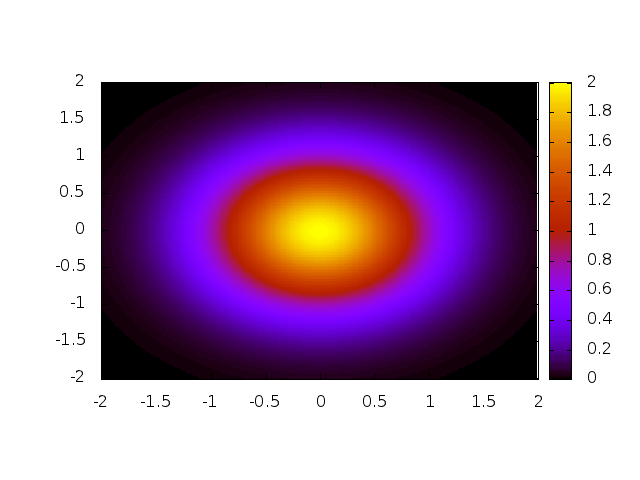
\includegraphics[scale=0.5]{deterioration1/fitnessLand.png}
  }
  \fbox{
    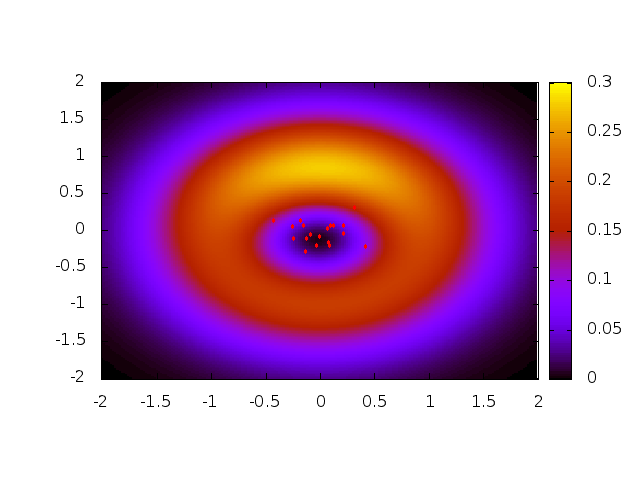
\includegraphics[scale=0.5]{deterioration1/deterioratedLandscape.png}
  }
  \caption{The result basic deterioration scheme with CMA 
  applied to unimodal function: $f(X) = 2e^{-(x^2 +y^2)}$.
  Optics paramters: $minPts=20, \epsilon=0.4$, algorithm: SGA, iterationCount=1}
  \label{det1}
\end{figure}

\begin{figure}
  \centering
  \fbox{
    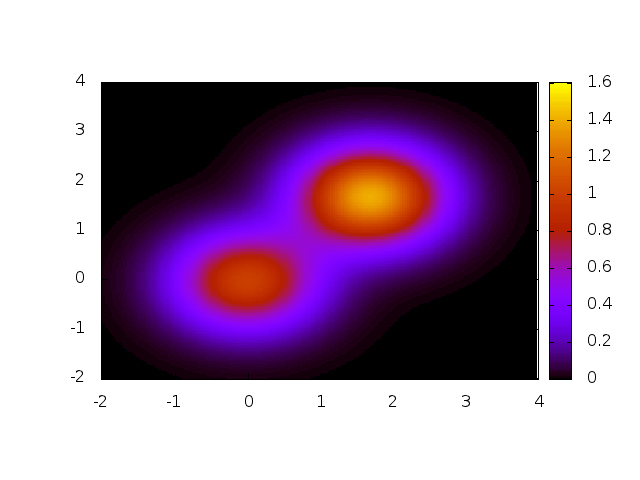
\includegraphics[scale=0.5]{deterioration3/fitnessLand.png}
  }
  \fbox{
    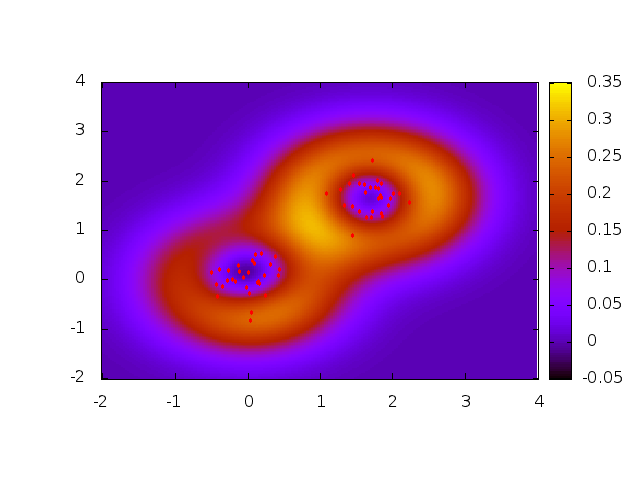
\includegraphics[scale=0.5]{deterioration3/deterioratedFitness.png}
  }
  \caption{The result basic deterioration scheme with CMA 
  applied to bimodal function: $f(X) = e^{-(x^2 + y^2)}+1.4e^{-((x-1.7)^2 +
  (y-1.7)^2)}$. Optics paramters: $minPts=20, \epsilon=0.4$, algorithm: SGA, iterationCount=2}
  \label{det2}
\end{figure}




\chapter{Tested Algorithms}
\label{TestedAlgorithms}


\section{HGS}
why HGS is well suited to our algorithm (suitable for clustering, fast
convergence in leaves)

\section{Tests}

\subsection{Benchmark functions}
uni, bi and multimodal functions

\subsection{Accuracy measures}
how many optimas have been found,
diagrams

\subsection{Efficiency measures}








\chapter{Implementation}
\label{Implementation}

\section{Architecture}

\section{Implementation in Java}
clean structure, good test coverage, 
modular architercture, extensible,

\subsection{Technologies}
Spring, Maven, JUnit, Mockito, JAMA, TDD approach

\subsection{Diagrams}
class diagrams, sequence diagrams





\chapter{Conclusions}
\label{Conclusions}

\section{Summary}

\section{Future Research}




%%%%%%%%%%%%%%%%%%%%%%%%%%%%%%%%%%%%%%%%%%%%
%%%%%%%%%%%%%%% Bibliograhpy %%%%%%%%%%%%%%%
%%%%%%%%%%%%%%%%%%%%%%%%%%%%%%%%%%%%%%%%%%%%

\bibliographystyle{alpha}

\begin{thebibliography}{10}
\bibitem{globalOpt}
\textit{Global Optimization Algorithms - Theory and Application} by Thomas Weise

\bibitem{optics}
\textit{OPTICS: Ordering Points To Identify the Clustering Structure}
by Mihael Ankerst, Markus M. Breunig, Hans-Peter Kriegel, Jrg Sander

\bibitem{esss}
\textit{Evolutionary search with soft selection} by A. Obuchowicz

\bibitem{foggo}
\textit{Foundations of global genetic optimization} by Robert Schaefer, Henryk
Telega

\bibitem{dataMining}
\textit{Introduction to Data Mining} by Tan, Steinbach, Kumar

\bibitem{probab}
\textit{Foundations of modern probability} by Kallenberg

\bibitem{nflt}
\textit{No Free Lunch Theorems for Optimization} by David Wolpert, William Macready

\bibitem{niching}
\textit{Niching Methods for Genetic Algorithms} by Samir W. Mahfound

\end{thebibliography}

\end{document}
